\documentclass[11pt,a4paper,oneside]{article}
\usepackage[utf8]{inputenc}
\usepackage{amsmath}
\usepackage{amsfonts}
\usepackage{amssymb}
\usepackage{graphicx}
\usepackage{color}
\usepackage {tikz}
\usetikzlibrary {er}
\usepackage[left=2.00cm, right=2.00cm, top=1.00cm]{geometry}
\graphicspath{{./}}

\begin{document}
	\title{DS 256 - Scalable Systems for Data Science \\ Assignment 1}
	\author{Shriram R. \\ M Tech (CDS) \\ 06-02-01-10-51-18-1-15763}
	\maketitle
	
	\section{Introduction}
	Distributed graph algorithms were implemented using Apache Spark RDD and Giraph vertex centric API. Strong and weak scaling experiments were performed using different public graph datasets to study the performance of these platforms in terms of different metrics. The following sections cover the experimental setup, plots and analysis in detail.  
	
	\section{Algorithms}
	The following four algorithms have been implemented for this assignment. Some brief notes on them is provided below,
	
	\subsection{Weakly Connected Components [1]}
	This is an iterative algorithm which converges once all the vertices in each weakly connected component reach the same value. The graphs were processed as undirected for this algorithm. The no. of steps would be roughly the diameter of the undirected graph.
	
	\subsection{Conductance [2]}
	This is the only single pass algorithm out of all four. The graphs were processed as undirected. In each execution, approximately $\frac{1}{3}^{rd}$ of the vertices were marked as IN in random fashion and the remaining were marked as OUT. This is to avoid a input vertex list for the experiments.
	
	\subsection{PageRank [3]}
	This algorithm is iterative and is made to run till convergence. The tolerance was set to $1\%$ and the weight was set to $0.85$ for all the experiments. The graphs were treated as directed graph. The no of iterations depend on the structure of the graph and it is guaranteed to converge. 
	
	\subsection{Spanning Tree [4]}
	This algorithm is also iterative and runs till the spanning tree is formed. The graphs were processed as undirected and a source vertex (Vertex ID = 1) is given as input to start the spanning tree search. The no. of iterations should be close to that of weakly connected components.
	     
    \section{Experimental Setup}
    
    \subsection{Hardware}
    Experiments were performed on a commodity cluster having 24 compute nodes. Each node has a 8-core AMD Opteron 3380 processor clocked at 2.6Ghz along with 32GB RAM and 2TB HDD and runs Ubuntu 16.04 LTS (64 bit) with Linux 4.4.0-139-generic. The nodes are connected through a Gigabit Ethernet switch.
    
    \subsection{HDFS and Apache Spark}
    The cluster is provisioned with Apache Hadoop 3.1.1. HDFS environment has a capacity of 1.32TB with block size 128MB, replication factor of 2 and heartbeat delay of 3s. The global configuration of Spark for all experiments is 3 executor cores per executor (containers) having 8GB of memory. The Driver memory was set to 512MB. Apache YARN was used to coordinate the job execution and jobs were submitted through cluster mode. Experiment specific detail if any is provided below.
    
    \subsection{Apache Giraph}
    The cluster is provisioned with Apache Giraph version 1.3.0. Each worker runs with 4 concurrent execution threads. The graphs are partitioned using Giraph's native hash partitioning. Checkpointing of the execution state and out-of-core execution was turned off for all experiments. The log level was set to debug and the Giraph metrics system was enabled. Apache YARN was used as the resource manager. YARN heap size was set to 12000 MB. 
    
    \subsection{Dataset}
    Experiments were run on the following three datasets. More datasets were not explored due to logistic constraints. The following table provides a summary of the graph datasets used,
    \begin{center}
    \begin{tabular}{|c|c|c|c|c|}
    	\hline 
    	\textbf{Dataset} & \textbf{Vertices $|V|$}  & \textbf{Edges $|E|$} & \textbf{Size (MB)} & \textbf{Input Format}\\
    	\hline
    	CITP & 3,774,768 & 16,518,948 & 280 & Edge List (TSV) \\
    	\hline
    	LIVJ & 4,847,571 & 68,993,773 & 1080 & Edge List (TSV) \\
    	\hline
    	ORKUT & 3,072,441 & 117,185,083 & 1769 & Edge List (TSV)\\
    	\hline
    \end{tabular}
    \end{center}
    	
    \section{Results \& Analysis}
    
    \subsection{Giraph - Strong Scaling}
    
    The following figures summarize the results of Strong Scaling experiments in Giraph on the above three datasets. Each algorithm was executed with four different configurations with $4$, $6$, $8$ and $10$ workers respectively with other parameters remaining constant. Note that each experiment was run only once successfully and the output values are taken directly. 
    
    The X-axis on the figures show no. of workers under each algorithm. Left Y-axis shows the time taken for different operations and the right Y-axis shows the scaling efficieny (E) in percentage computed using the following formula where $n$ is no. of workers and $t_n$ is time taken using $n$ workers,
    
    $$E_n = \frac{t_4 * 4}{t_n * n}*100\%$$
    
    The compute time includes the time spent on computation and the I/O time includes the time spent on sending messages across the workers during each superstep. Note that combiners were not used to combine messages and so the time taken is for all the generated messages to be transferred.
    
    The configurations were chosen such that the algorithms would run into completion in reasonable amount of time without causing issues.
    
    \begin{center}
    	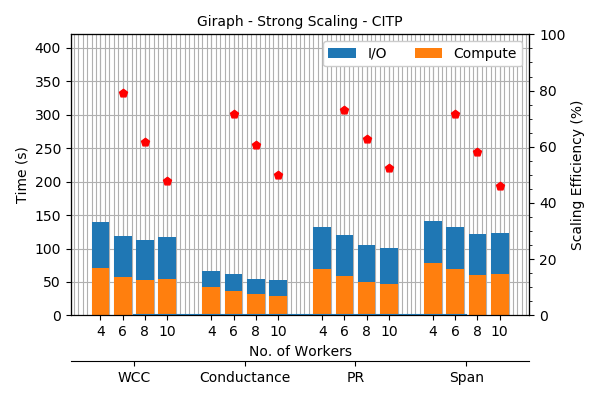
\includegraphics[scale=0.5]{1.png} \\	
    	Figure 1 - Giraph - CITP - Strong Scaling	
    \end{center}

    \begin{center}
    	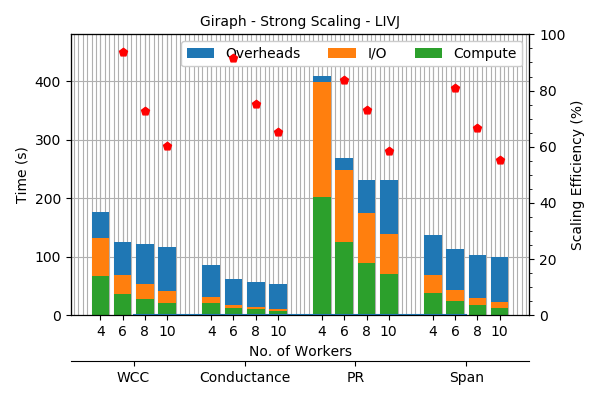
\includegraphics[scale=0.5]{2.png} \\
    	Figure 2 - Giraph - LIVJ - Strong Scaling		
    \end{center}

    \begin{center}
    	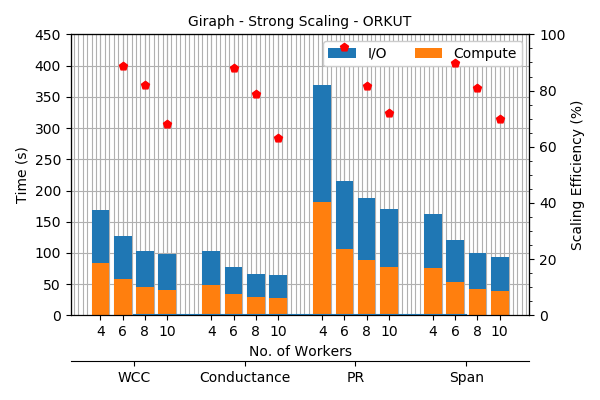
\includegraphics[scale=0.5]{3.png} \\
    	Figure 3 - Giraph - ORKUT - Strong Scaling		
    \end{center}

    
    \pagebreak

    It can be observed that the total time generally decreases when the no. of workers is increased for all the datasets and all the algorithms. However it must be noted that the scaling efficieny is low ($50 -90 \%$) and keeps decreasing as the workers are increased. This is as expected and clearly shows that the algorithms do not strongly scale in Giraph system.
    
    Conductance takes the least time of all the four algorithms. This as expected since it is a single pass algorithm with most of the values written directly to the master aggregator. It is followed by Weakly Connected Components (WCC), Spanning Tree (Span) and PageRank (PR). PR takes most time in general since in every generation all the vertices send messages to all its neighbours. 
    
    Another interesting observation is that the I/O time is fairly equal to compute time in most of the cases. This motivates the need for using combiners to reduce the no. of messages transferred across the nodes. Also, graph partitioning plays an important role in reducing the no. of internode messages by reducing the no. of edge cuts. Hash partitioning used in this case does not optimize for edge cuts.
    
    Across the different datasets, the time taken does not propotionally varies in interms of no. of edges or vertices for the same algorithm and configuration. 
    
    \subsection{Giraph - Weak Scaling}
    
    The figure below summarizes the result of weak scaling experiment in Giraph. CITP was used as the base case with 1 worker. LIVJ and ORKUT were used on larger no. of workers (4 and 7 respectively) by keeping the edges per worker constant. This decision was made since the compute in each vertex essentially boils down to no. of edges. PR for 1 worker could not be completed successfully due to runtime error and so it is not shown.
    
    The X-axis shows the no. of workers. The left Y-axis shows the time taken and the right Y-axis shows the scaling efficieny. The scaling efficieny E was calculated using the below formula,
    
    $$E_n = \frac{t_1}{t_n}*100\%$$

    \begin{center}
    	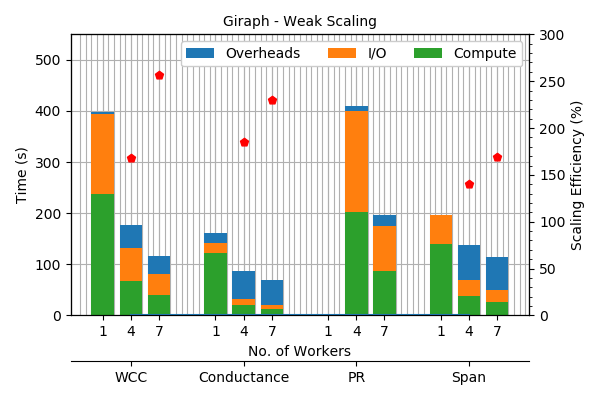
\includegraphics[scale=0.5]{4.png} \\
    	Figure 4 - Giraph - Weak Scaling	
    \end{center}

    It can be observed that the system shows weak scaling for all algorithms. The scaling efficieny indicates that it is superlinear. This is because that graphs used for each worker count is different in terms of degree distribution, diameter, topology etc. all of which could affect the time taken in addition to the edge count.
        
    \section{References}
    \begin{list}{}{}
    	\item
    	\item
    \end{list}  
    
\end{document}